\subsection{Image Processing}
We mainly take into account two aspects when choosing the concept for image
processing: precision and adaptability. According to our customer requirements,
we need to reach high efficiency in annotation for autonomous driving scene. An
accurate annotation hint during preprocessing will improve a lot in the overall
labeling efficiency. Besides, in autonomous driving scene we may have images
with various complex conditions, so we need the image processing process to
have a high adaptability to work well in different conditions. Since we are not
restrained in computing resources, and it is less possible that computation
time becomes the critical path in our interacting system, we do not require our
concept to be computational efficient. Based on the concept generation in
section 5, we have 3 possible approaches:

\begin{enumerate}
    \item Deep learning: using deep neural network models to detect and
classify objects
        \begin{itemize}
            \item[$\blacktriangleright$] \textbf{Advantages}
                \begin{itemize}
                    \item High Accuracy. The accuracy of a well-trained model
can reach 95\% in a similar task like object detection.
                    \item High Adaptability. Deep learning works well even in
complex environments such as nighttime or heavy traffic.
                \end{itemize}
            \item[$\blacktriangleright$] \textbf{Disadvantages}
                \begin{itemize}
                    \item Time and resource consuming. Training a neural
network from the very beginning requires hardware and takes a lot of time to
complete.
                    \item Dataset required. To train a deep learning model, it
is necessary to find or create a suitable dataset for it. Otherwise too few
data will lead overfitting.
                    \item Not flexible. Modification on model structure or
adding more classes to detect requires relabeling dataset and retraining.
                \end{itemize}
        \end{itemize}
    \item Traditional Machine Learning: using SVM and other traditional ML
techniques
        \begin{itemize}
            \item[$\blacktriangleright$] \textbf{Advantages}
                \begin{itemize}
                    \item Adaptability. It can be used even when images has
been scaled or rotated.
                    \item Fast training. Compared to deep learning, limited
parameters are involved in training, thus reducing the training time.
                \end{itemize}
            \item[$\blacktriangleright$] \textbf{Disadvantages}
                \begin{itemize}
                    \item Not very accurate. Especially with a large number of
classes, the accuracy drops.
                    \item It can be difficult to distinguish similar objects
using traditional techniques. Also, it may be sensitive to different lighting
conditions.

                \end{itemize}
        \end{itemize}
    \item Image Processing: using SIFT, HOG techniques
        \begin{itemize}
            \item[$\blacktriangleright$] \textbf{Advantages}
                \begin{itemize}
                    \item No training needed. The algorithm can work instantly.
                \end{itemize}
            \item[$\blacktriangleright$] \textbf{Disadvantages}
                \begin{itemize}
                    \item Require good image quality to get feature keypoints
to detect.
                    \item Low accuracy when images contain too many things to
detect.
                \end{itemize}
        \end{itemize}
\end{enumerate}
By comparison, deep learning stands out in precision and adaptability when
compared to the traditional machine learning and image processing methods. To
resolve the problem of computing resources, we decide to use pretrained models
to bypass the problem. Therefore, we select deep learning as the approach for
image processing. We summarize the selection process in the scoring matrix
(Table \ref{tab:SelectionML}).

\begin{table}[htbp!]
    \centering
    \begin{tabular}{|c|c|c|c|c|} \hline
        Demanded Quality & Deep Learning & \makecell{Traditional\\Machine
Learning} & Image Processing \\ \hline
        Precision & 5 & 4 & 2 \\ \hline
        \makecell{Independence from\\Computing Resource} & 2 & 3 & 4 \\ \hline
        Adaptability & 4 & 3 & 2 \\ \hline
        \textit{Sum of total} & 11 & 10 & 8 \\ \hline
    \end{tabular}
    \caption{Scoring Matrix of Concept Selection in Image Preprocessing. Scores
are out of 5.}
    \label{tab:SelectionML}
\end{table}

\subsection{Major Deep Learning Architectures Selection}
For the deep learning models, we are primarily trading off between Bounding Box
accuracy, class prediction accuracy, inference speed, model recall rate, and
false positive rate. We put extra weight on the inference speed, since it is
our major requirement for labeling efficiency.  Based on that, we figured out a
plot as shown in Fig. \ref{fig:yolo_comp}. Besides, we took into consideration
the following factors when doing concept selection:



\begin{itemize}
    \item For different environment lighting conditions, we need to be
invariant.
    \item For unbalanced numbers of samples in different classes, we need to do
augmentation to create an unbiased result
    \item Traffic signs in the image may have different sizes and resolutions.
Our model needs to be invariant to scales and resolutions.
    \item For better detection accuracy for multi-class, we need to enhance
some features in the input.
\end{itemize}

\subsubsection{Object Detection}

The object detection part of our deep learning architecture is based on YOLOv3.
Besides, we also have other choices such as Retina-Net since it is also among
the state of art architectures. The advantages and disadvantages of these
methods are listed as follows:
\begin{figure}[h!]
  \centering 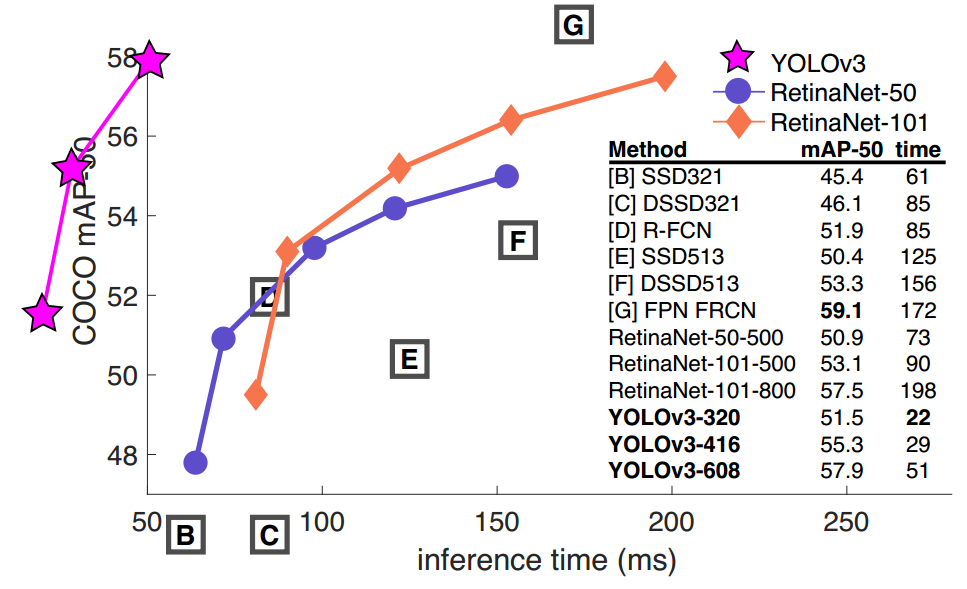
\includegraphics[width=\linewidth]{lyy_YOLOv3_compare.png}
  \caption{Concept selection for object detection. The inference speed and
accuracy on COCO test data are compared. We see from the figure that YOLOv3
performs best in terms of inference time}
  \label{fig:yolo_comp}
\end{figure}

\begin{enumerate}
    \item YOLOv3:
        \begin{itemize}
            \item[$\blacktriangleright$] \textbf{Advantages}
                \begin{itemize}
                    \item Relatively high recall rate. The change from
\texttt{Softmax} to \texttt{Sigmoid} makes the multi-class prediction more
accurate.
                    \item Fast inference speed. 10x of RetinaNet under the same
accuracy requirement.
                    \item Low false positive rate in object detection when
using DarkNet as backbone. It is due to its ability to learn the difference
across scales.
                \end{itemize}
            \item[$\blacktriangleright$] \textbf{Disadvantages}
                \begin{itemize}
                    \item Low recall rate when an object is unseenable.
                    \item Lower accuracy for bounding box localization.
                    \item Not able to identify human pose, or more detailed
information about objects. For example, the current YOLOv3 can only identify
stop signs as traffic signs.
                \end{itemize}
        \end{itemize}
        \item Retina-Net
        \begin{itemize}
            \item[$\blacktriangleright$] \textbf{Advantages}
                \begin{itemize}
                    \item Relatively higher accuracy for object classification
since it is region-based
                    \item Better bounding box localization
                    \item Higher recall rate when different classes are
presented.
                \end{itemize}
            \item[$\blacktriangleright$] \textbf{Disadvantages}
                \begin{itemize}
                    \item Higher false positive rate.
                    \item Not able to identify human pose, or more detailed
information about objects.
                \end{itemize}
        \end{itemize}
\end{enumerate}

\begin{table}[htbp!]
    \centering
    \begin{tabular}{|c|c|c|} \hline
        Demanded Quality &\makecell{YOLOv3} & \makecell{Retina-Net} \\ \hline
        \makecell{BBox \\ Accuracy} & 4 & 5  \\ \hline
        \makecell{Classification\\ Accuracy} & 4 & 4  \\ \hline
        Inference speed  & 5 & 3  \\\hline
        False Positive rate & 4 & 5 \\ \hline
        Recall rate  & 5 & 4 \\ \hline
        \textit{Sum of total} & 22 & 21 \\ \hline
    \end{tabular}
    \caption{Scoring Matrix of Concept Selection in Object detection of image
preprocessing module. Scores are out of 5.}
    \label{tab:obj_detec_comp}
\end{table}


\subsubsection{Human-pose Estimation}
For human-pose estimation, we primarily compared some Top-down approaches
(Convolutional Pose Machines \cite{Wei_2016} and Single Shot MultiBox Detector
\cite{Liu_2016}) versus Part-Affinity Field.
The seminal work of Zhe Cao et al. \cite{Cao2016Realtime} used Pars Affinity
Field (PAF), jointly learning parts detection and parts association as a
down-top approach. Their properties are compared in the following table
\ref{tab:obj_detec_comp}.

\begin{table}[htbp!]
    \centering
    \begin{tabular}{|c|c|c|} \hline
        Demanded Quality &\makecell{Top-down\\ approach} & \makecell{PAF} \\
\hline
        \makecell{Average Precision} & 4 & 5  \\ \hline
        \makecell{Accuracy\\ (Occluded joints)} & 4 & 5  \\ \hline
        \makecell{Accuracy\\ (multi-person)}  & 3 & 5  \\\hline
        \textit{Sum of total} & 11 & 15 \\ \hline
    \end{tabular}
    \caption{Scoring Matrix of Concept Selection in human pose estimation
module. Scores are out of 5.}
    \label{tab:SelectionPre}
\end{table}

From the table of comparison, we can clearly see that PAF offers an advantage
over the traditional top-down approaches, especially under occluded scenario
and multi-person scenes, which is suitable for our design concept.

\subsection{GUI Design}
We mainly take into account three aspects when choosing the concept for GUI
Design: portability, usability and existence of similar software. Based on our
requirements, we need to produce both a standalone software and an online
deployment. We also need to implement various functions in GUI to ease the
users during the annotation process, so we would like our GUI library to
provide convenience in implementation. High portability means that less efforts
are needed when deploying our standalone software online. If there are existing
open source software with similar functionality using a certain library, we can
build our software upon it and save much effort. Usability mainly consists of a
steady learning curve and a powerful API that can boost coding efficiency.
Among the three candidates, Qt and WxWidgets have a high portability between
various platforms and programming languages. We can find existing software
using Qt and Tk library. Qt has its own developing environment that can ease
the process of coding and Tk has a powerful API. Since Qt satisfies all of our
requirements, we select it as our concept for GUI Design. We summarize the
selection process in the scoring matrix (Table \ref{tab:SelectionUI}).

\begin{table}[htbp!]
    \centering
    \begin{tabular}{|c|c|c|c|c|} \hline
        Demanded Quality & Qt & WxWidgets & Tk \\ \hline
        Portability & 5 & 4 & 2 \\ \hline
        \makecell{Community Support} & 4 & 2 & 4 \\ \hline
        \makecell{Simplicity of Coding Logic} & 5 & 3 & 2 \\ \hline
        \textit{Sum of total} & 14 & 10 & 8 \\ \hline
    \end{tabular}
    \caption{Scoring Matrix of Concept Selection in GUI Design. Scores are out
of 5.}
    \label{tab:SelectionUI}
\end{table}

\subsection{Server Selection}
\begin{table}[htbp!]
    \centering
    \begin{tabular}{|c|c|c|c|} \hline
        Demanded Quality & Nginx & Apache &Flask\\ \hline
        Data Transmission Speed & 5 & 4 & 3\\ \hline
        \makecell{Multi-server Scalability} & 4 & 3 & 4 \\ \hline
        \makecell{Rewrite Frequency} & 4 & 5 & 5\\ \hline
        \textit{Sum of total} & 13 & 12 & 12\\ \hline
    \end{tabular}
    \caption{Scoring Matrix of Concept Selection in Online Deployment Server.
Scores are out of 5.}
    \label{tab:SelectionServer}
\end{table}

We mainly take into account three aspects when choosing the concept for online
deployment (server): data transmission speed, multi-server adaptability, and
rewrite frequency. Data transmission speed is critical to boost label
efficiency, which is a major requirement in our QFD chart. The second is
multi-server environment, which means if our environment can be deployed on
multiple servers without much effort. The third is rewrite frequency, which
means if our URL can be reset and redirected. Websites are personalized to meet
their business needs when using Nginx, and URL rewriting is almost a must for
every website.

Apache, Flask and Nginx are the three most common open source web servers in
the world. All of the solutions are capable of handling diverse workloads and
working with other software to provide a complete web stack. In our project,
the users responsible for labeling should be able to download the image with
the preprocessed data label quickly. The user will first download the
preprocessed data from the server, and after manually modifying the labels,
they can upload the image back to the server. As the request is posted, the
server should be able to respond in a short time.

Since we need fast data transmission to meet with the requirement of efficient
labeling, we need to have a server with fast static resource transmission.
Besides, we do require multiple servers or load-balancing when we have a large
number of datasets. Nginx's URL rewriting rules are not as straightforward as
Apache, and the logic is relatively complicated. But we have medium rewrite
frequency, so at last, we choose Nginx over Apache and Flask.

We summarize the selection process in the scoring matrix (Table
\ref{tab:SelectionServer}).
